\begin{frame}{About Me}
\note{
    I hold a Ph.D. in Computational Engineering, a field that bridges computation and practical applications.

    \scriptsize{
      Over the years, I've played various roles. Let's take a walk down memory lane:
      My journey began as a Software Developer at Valka, which later evolved into Marel. I contributed to their revolutionary waterjet cutter's software.
      Venturing into databases, I became an SQL Consultant at AGR.
      After defending my PhD, my next destination was deCODE genetics, diving into genetic research and long-range sequencing.
      The gaming world beckoned after COVID, and I joined CCP Games as a Data Scientist.
      Travelshift saw me as their Head of AI Research, where I tackled challenges similar to those during my PhD days.
      \textbf{Presently}, I have the privilege of mentoring young minds as an Assistant Professor in the Industrial Engineering Department at the University of Iceland.
    }

    \begin{itemize}
        \item A notable highlight of my career was my talk on the \emph{Legend of the Ice People} at Reykjavík Databeers. This talk drew inspiration from a literary podcast I hosted, \emph{ÍSKISUR}. A modern take on literary analysis, it was a thrilling experience.
        \item On being invited to this distinguished conference to discuss ÍSFÓLKIÐ, many might deem it 'trivial'. Yet, as we're about to delve into, ÍSFÓLKIÐ is far from mundane as the data will show.
    \end{itemize}
}

I am a \emph{Ph.D.} in Computational Engineering.
\vspace{1em}
\begin{columns}[T] % alignment of columns
  \begin{column}{0.6\textwidth} % adjust width to your liking
    Past Roles:
    \begin{itemize}
      \item Software Developer at Valka
      \item SQL Consultant at AGR
      \item Research Scientist at deCODE genetics
      \item Data Scientist at CCP Games
      \item Head of AI Research at Travelshift
    \end{itemize}
  \end{column}

  \begin{column}{0.35\textwidth} % adjust width to your liking
      \begin{exampleblock}{Current Role:}
        \emph{Assistant Professor} in the Industrial Engineering Department at the University of Iceland
      \end{exampleblock}
  \end{column}
\end{columns}

  \vfill
  \begin{block}{Signature Talk}
      Analysis of \emph{Legend of the Ice People} a.k.a. \emph{ÍSFÓLKIÐ} for Reykjavík Databeers \#6.

      \vspace{0.5em}

      Inspired by the literary podcast I co-hosted, \emph{ÍSKISUR}.
  \end{block}
\end{frame}


\begin{frame}{A Surprising Insight}
\note{
  \begin{itemize}
    \item When I presented at Databeers last June, I planned for a 7-min lightning talk.
    \item However, the audience's reaction took me by surprise.
    \item They were intrigued by the data-driven angle I took on ÍSFÓLKIÐ.
    \item Many expressed astonishment at the idea of applying data-driven approaches to literature.
    \item The discussions were so engaging that, with permission, we went well over time, turning that brief talk into a 45-minute in-depth discussion.
    \item So if there's one key \textbf{takeaway} from my experience, it's this:
    Data is all around us. With the right perspective, we can find and interpret data in the most unexpected domains.
    \item Be open to data, and it can unlock fresh insights and lively discussions, as I found out!
  \end{itemize}
}

\begin{columns}[T]

  \begin{column}{0.6\textwidth}
    What surprised most about my presentation at \emph{Reykjavík Databeers} was the audience's reaction:
    \begin{itemize}[<+->] % <+-> will animate the items to appear one-by-one
      \item They didn't expect a data-driven angle to \emph{ÍSFÓLKIÐ}.
      \item Astonished by \emph{several} data-driven approaches to literature.
      \item Analytical framework shed new light and perspectives.
    \end{itemize}
  \end{column}

  \begin{column}{0.4\textwidth}
    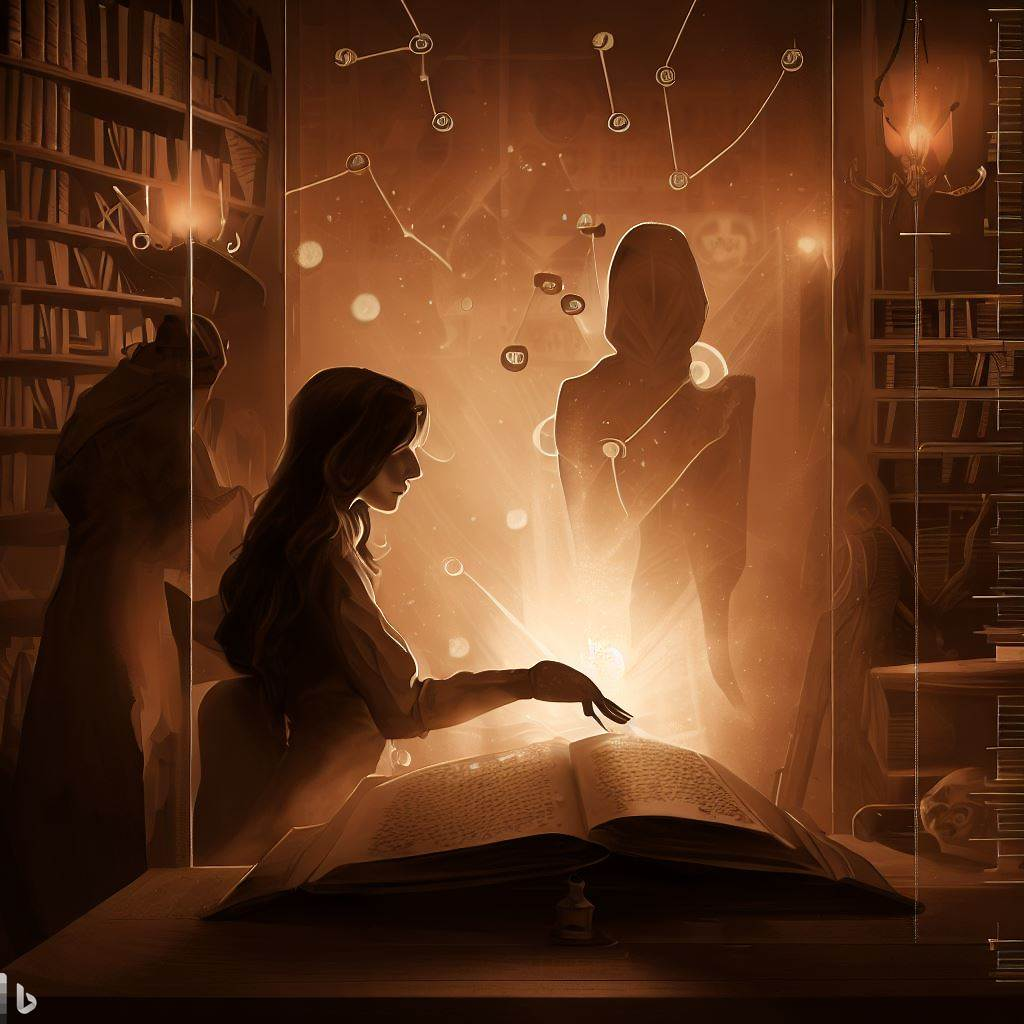
\includegraphics[width=\textwidth]{../figures/dalle-insights} % Consider an image that represents surprise or insight.
  \end{column}

\end{columns}

\vspace{0.5em}

\begin{block}{Take-Home Message}
Anything can be data-driven with the right mindset. Data is everywhere; it's about looking for it and using it. Embrace data for fresh insights, even in unexpected domains.
\end{block}

\end{frame}


\begin{frame}{Backstory: From Cat Memes to Podcasts} \note{
In 2012, I stumbled upon the world of \textbf{internet cats} and was immediately \textit{captivated}.
It began innocently enough: I'd seek out \textbf{quirky cat memes} to share on my social platforms.
But soon, it became more than just a hobby. My friends began \textit{discreetly} forwarding me cat images,
and I'd then share them with the world. Without even realizing it, I became a well known \underline{internet cat lady}.

\bigskip  % A pause here for a slight change in topic

By 2016, I discovered a podcast named \textbf{My Dad Wrote A Porno}. It was both \textit{hilarious} and spellbinding.
Inspired by their creativity, my friends and I wanted to start our own show.
But we faced a problem: none of our parents wrote erotic fiction. So, we \textbf{improvised} and decided to read \emph{ÍSFÓLKIÐ},
putting our own twist on it.

\bigskip  % Another pause for a change in topic

To incorporate my love for cats, I introduced a special segment at the end of each episode titled
\emph{Internet Cat of the Week}. And that's how two of my passions \underline{converged}.
    }
    \begin{itemize}
        \item 2012: Became the internet cat lady -- Memes $\Rightarrow$ Friends' Cat pics.
        \item 2016: Inspired by \emph{My Dad Wrote A Porno} podcast.
        \item Solution: Read \emph{ÍSFÓLKIÐ} with our twist.
        \item Special Segment: \emph{(Internet) Cat of the Week}.
    \end{itemize}
    \vfill


\begin{columns}
    \begin{column}{0.8\textwidth}
        \begin{exampleblock}{TL;DL: My Dad Wrote a Porno (2015--)}
            A 3-time Webby Award-winning comedic podcast where host Jamie Morton reads his father's amateur erotic novel. With friends James Cooper and Alice Levine, they hilariously dissect awkward, improbable tales blending family and risqué fiction.
        \end{exampleblock}
    \end{column}
    \begin{column}{0.2\textwidth}
        
\includegraphics[width=\textwidth]{../figures/my-dad-wrote-a-porno}
    \end{column}
\end{columns}


\end{frame}

\begin{frame}{About ÍSKISUR}
    \note{
      \textbf{Introduction to ÍSKISUR:}
      ÍSKISUR is a rather unique podcast, combining two things many wouldn't expect to find together: literature and, believe it or not, cats. Each episode we dive into the world of \emph{The Legend of the Ice People} by Margit Sandemo. This series is filled with both erotic and surreal elements, making it a treasure trove for lively discussions.

      \textbf{Episode Structure:}
      But our podcast doesn't end with just discussing the book. As a nod to my personal fondness for cats, every episode concludes with a delightful segment on internet cats.

      \textbf{Graphics and Podcast Members:}
        Now, if you look to your left, you'll see an iconic image from the Internet Cat Festival held back in 2013. This memorable meeting between Grumpy Cat and Lil Bub truly epitomizes the fun spirit of our show.
        And to your right is our official podcast image on Storytel. It features myself alongside my amazing co-hosts Birna and Kristín.
        \textbf{Disclaimer}: despite our deep dives into the book series, none of us claim to be actual cats or literary experts.
    }
    \begin{columns}[T]
        \begin{column}{0.55\textwidth}
            \begin{itemize}
                \item A literary and feline entertainment podcast*
                \item Discuss the erotic and surreal book series \emph{The Legend of the Ice People} by Margit Sandemo
                \item Each episode covers part of a book from the series and concludes with a segment on internet cats
            \end{itemize}
            \vspace{12pt}

            \centering
            
\includegraphics[width=.7\textwidth]{../rek-data-beers/figures/internet-cats}
            \tiny{via @iamlilbub}

            \scriptsize{Grumpy Cat first meeting Lil Bub\\Internet Cat Festival, 2013}
        \end{column}x
        \begin{column}{0.45\textwidth}
            \centering
            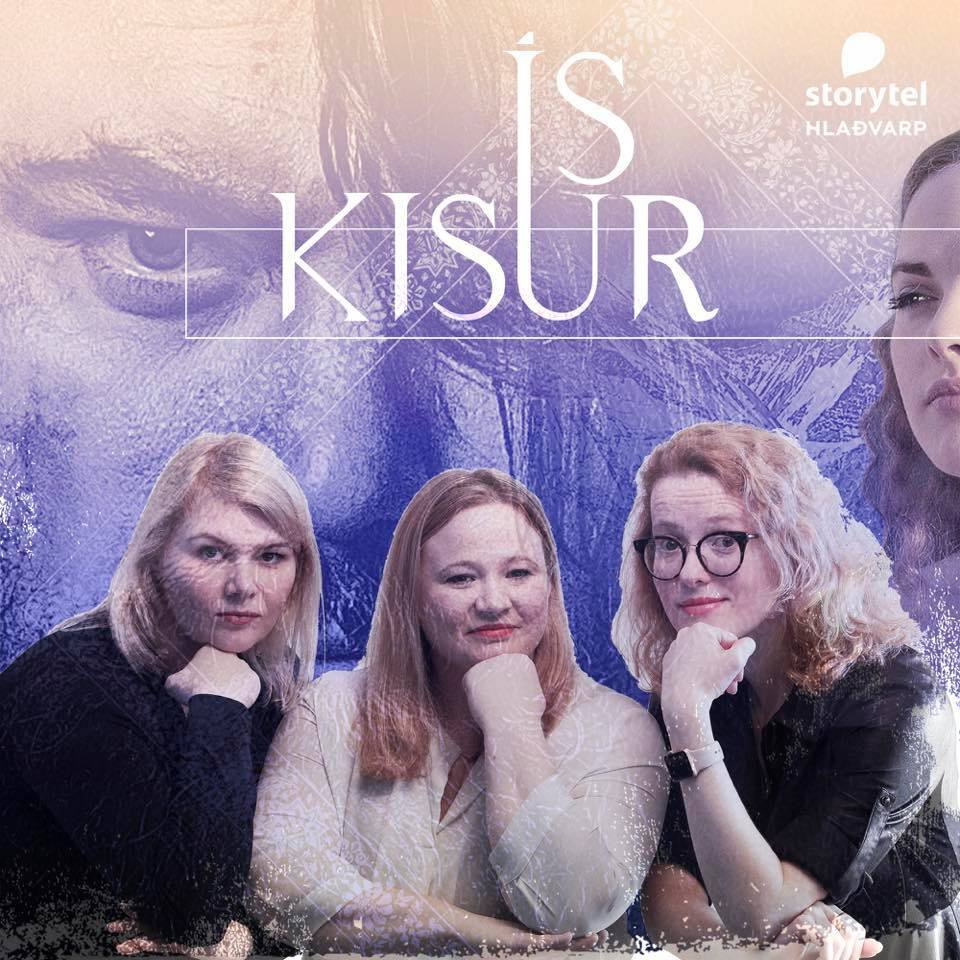
\includegraphics[width=\textwidth]{../rek-data-beers/figures/podcast_image.jpg}
            \vfill
            Birna, Kristín, and dr.~Helga\\
            \vspace{12pt}
            \footnotesize{*\textit{None of the hosts are actually cats or literary experts.}}
        \end{column}
    \end{columns}
\end{frame}

\begin{frame}{About ÍSFÓLKIÐ}
    \note{
    \begin{itemize}
        \item ÍSFÓLKIÐ: A 47-volume family saga in historic Scandinavia, filled with mystical elements.
        \item Central is Silja and her family, marked by an age-old curse from Þengill.
        \item While Silja's bond with Þengill the Good deepens the curse's influence, their descendants wrestle with its implications.
        \item The family's enduring struggle is with Þengill the Bad, culminating in an epic confrontation.
        \item Throughout, spirits and mystical mandrake root play crucial roles, assisting the family.
    \end{itemize}
    }

    \begin{columns}[T]
        \begin{column}{0.65\textwidth}
            \begin{itemize}
                \item Epic 47-volume tale set in historic Scandinavia with fantasy elements.
                \item The tale revolves around a \emph{curse} originating from malevolent Þengill.
                \item Silja, an ordinary woman, becomes intertwined with the curse through Þengill the Good.
                \item Their offspring, destined to face Þengill the Bad's rising evil, represent each book's focus.
                \item Culmination: The family's ultimate confrontation with Þengill the Bad.
                \item Spirits and mandrake root: Mysterious aids interwoven into the narrative.
            \end{itemize}
        \end{column}

        \begin{column}{0.35\textwidth}
            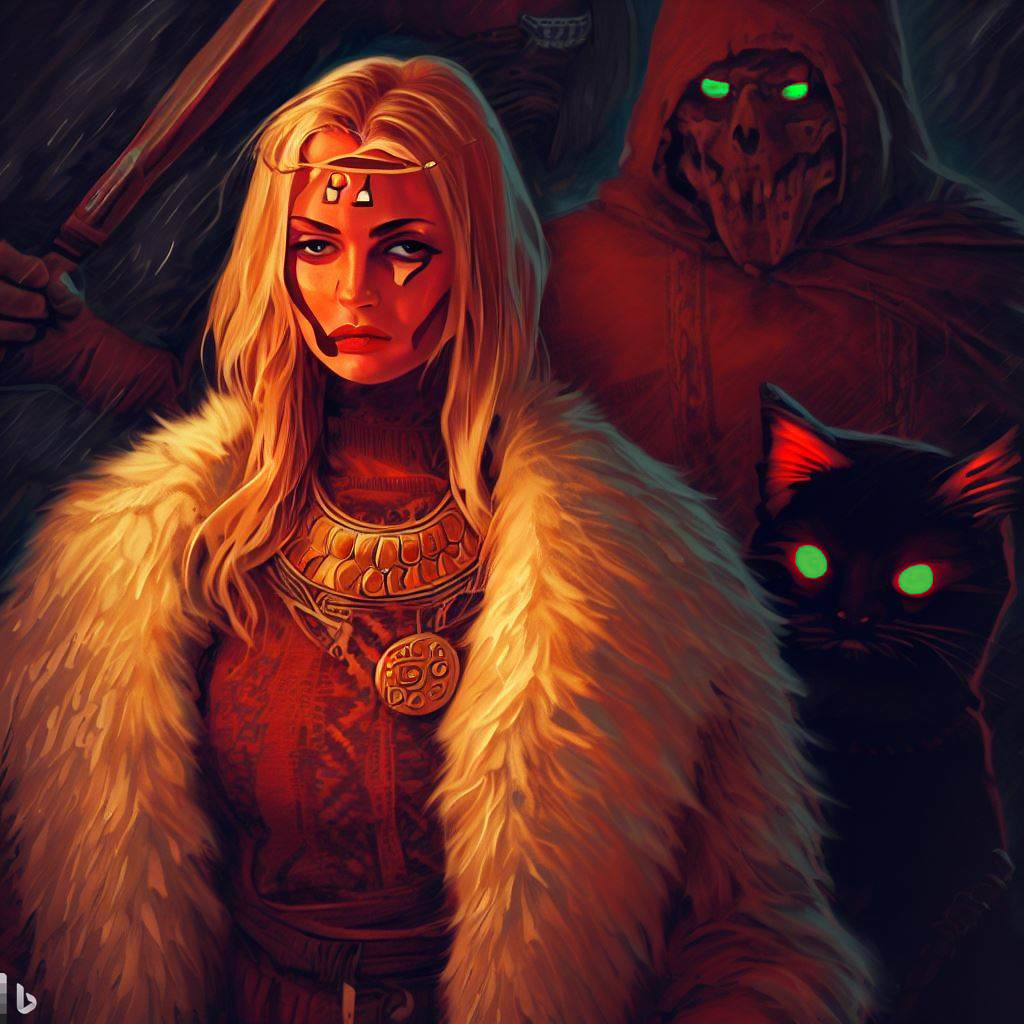
\includegraphics[width=\textwidth]{../figures/dalle-ísfólkið}
            {\scriptsize\begin{itemize}
                \item \emph{Silja}: Innocent matriarch of the cursed family.
                \item \emph{Þengill the Good}: Bearer of the curse, forsakes celibacy for Silja.
                \item \emph{Þengill the Bad}: Ever-strengthening evil antagonist.
            \end{itemize}}
        \end{column}
    \end{columns}
\end{frame}

\begin{frame}{Exploring Different Formats}
\note{
\scriptsize{
    \textbf{The Written format:}

    During the 80s, the \emph{Ísfólkið} became more than just literature; it evolved into a cultural phenomenon, deeply embedding itself in the collective consciousness of a generation.
    Its impact extended beyond the pages, shaping real-life naming trends in Iceland. Names like \emph{Villimey}, \emph{Viljar}, and \emph{Heikir} were previously non-existent, absent from the Icelandic census, until their introduction through the series.
    Similarly, after their respective book releases, names such as \emph{Sunna}, \emph{Silja}, \emph{Þengill} and \emph{Eldar} witnessed a significant surge in popularity, testament to the series' influence.

    Its relevance persisted, prompting a re-translation in 2007 for newer readers.

    \textbf{The Audio format:}
Storytel is a digital subscription service that offers audiobooks and e-books to its users on a global scale.
    \begin{itemize}
        \item ÍSFÓLKIÐ, introduced in 2017, quickly became titans on Storytel, showcasing the series' undying charm.
        Their widespread success transformed them into one of the most sought-after listens on the platform.
        \item ÍSKISUR, initially a simple bookclub discussion among friends on Alvarpið, the podcast breathed a fresh, candid perspective into the series.
        \item Recognizing the value and its potential, Storytel approached us. Moved by the soaring popularity of the audiobooks, they offered professional editing, and a soundstage for recording, elevating our small DIY project to professional production standards.
    \end{itemize}
}
}


  \begin{columns}[T] % alignment of columns
    \begin{column}{0.32\textwidth}
        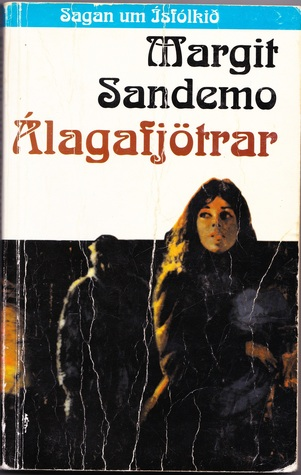
\includegraphics[width=.48\textwidth]{../figures/álagafjötrar_margit}
        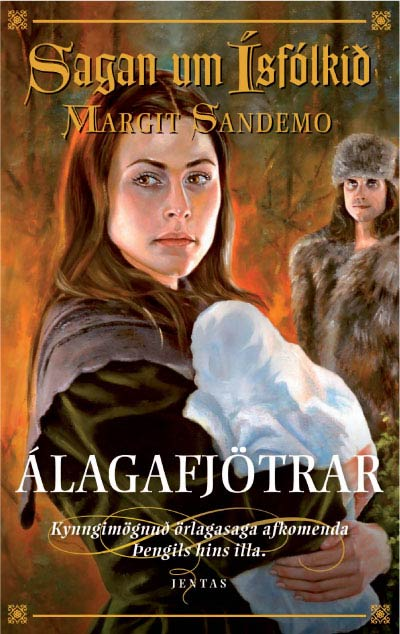
\includegraphics[width=.48\textwidth]{../figures/álagafjötrar_jentas}\\
      \textbf{The Written Books}
      \begin{itemize}
          \item 80s cult phenomenon.
          \item Re-translated in 2007.
          \item Influenced children's names.
      \end{itemize}
    \end{column}
\pause
    \begin{column}{0.32\textwidth}
        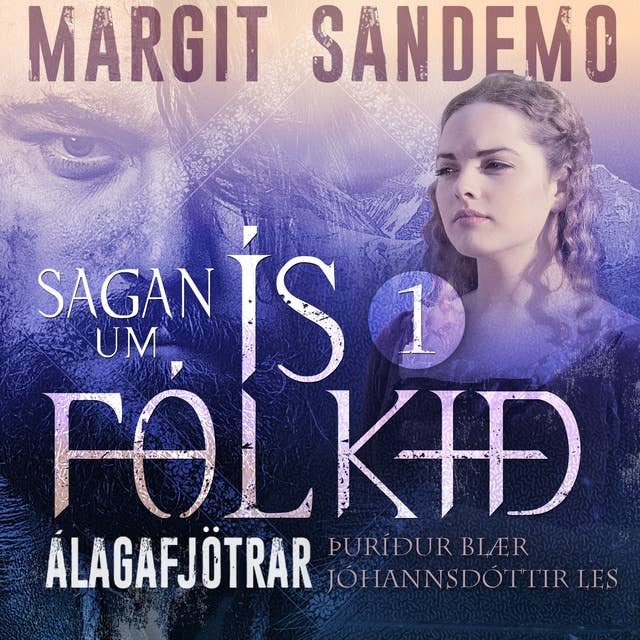
\includegraphics[width=\textwidth]{../figures/álagafjötrar_storytel}\\
      \textbf{The Audio Books}
      \begin{itemize}
        \item Top content on \emph{Storytel}.
        \item Widely listened to.
      \end{itemize}
    \end{column}
\pause
\begin{column}{0.32\textwidth}
  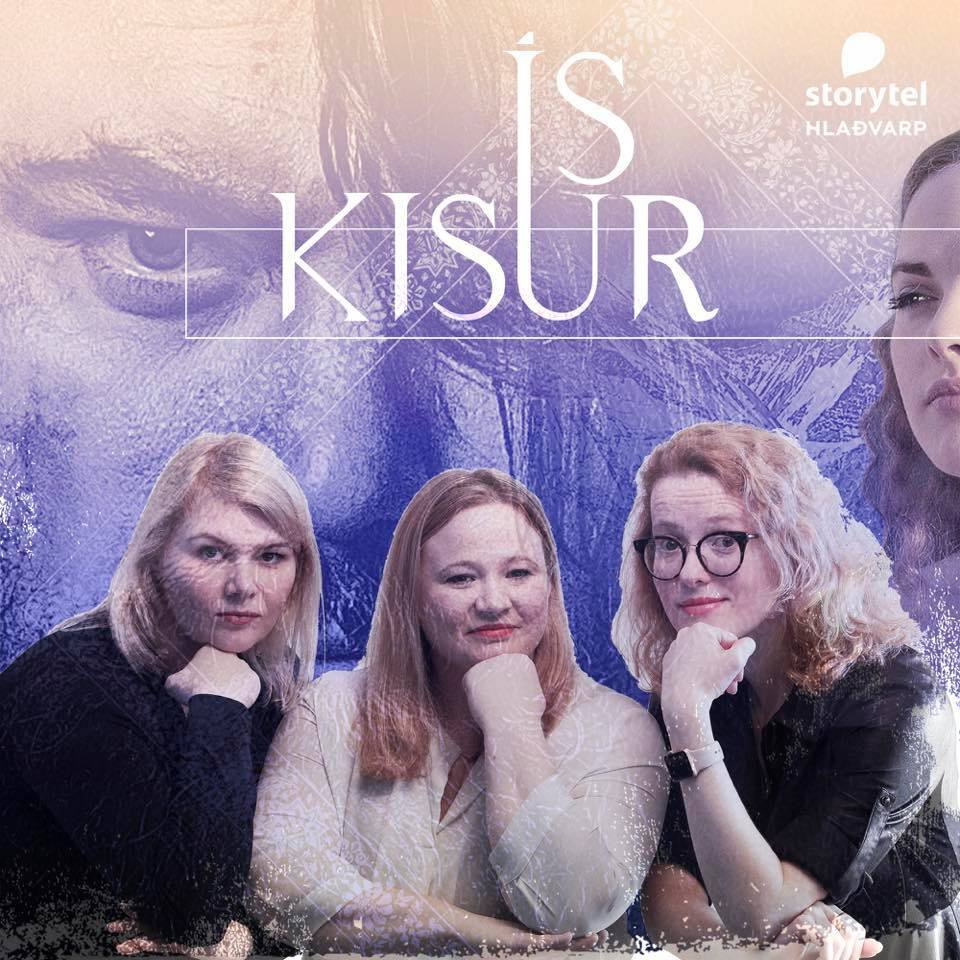
\includegraphics[width=\textwidth]{../figures/álagafjötrar_ískisur}\\
      \textbf{The Podcast}
      \begin{itemize}
        \item Small friend-led bookclub.
        \item Started on \emph{Alvarp Nútímans}.
        \item Moved to \emph{Storytel}.
      \end{itemize}
    \end{column}
  \end{columns}
\end{frame}


\begin{frame}{Timeline for the Legend of the Ice Cat-People}
\note{
\tiny{
    \textbf{Visual Overview:}
    The slide visually encapsulates the publication journey of both the written form and its newer audio adaptations.
    There are several life events annotated on the timeline which I'll further discuss and expand upon in subsequent sections.

    \textbf{Upper half: Book Series}
    \begin{itemize}
        \item Showcases the staggered release of the entire 47-part saga in Iceland.
    \end{itemize}

    \textbf{Lower half: Audio Adaptations}
    \begin{itemize}
        \item The journey began in earnest in fall 2016, when initial podcast episodes were recorded, but remained unreleased as we refined our production skills.
        \item ÍSKISUR made its debut on Alvarpið's 3rd anniversary in 2017, our podcast was featured alongside renowned titles such as Hefnendur and Englaryk.
        \item It's noted, this is before the major e-book release on Storytel. I like to think of ourselves as trendsetters.
        \item Although a hiatus intervened due to scheduling clashes and health issues, our passion project took a fortunate turn in 2019. Storytel recognized the podcast's potential and extended a collaboration offer. This meant not only compensation for our efforts but also relief from cumbersome post-production tasks, as we were living in different part of the country, and later different countries.
        \item With Storytel continuing the distribution of the audiobooks into fall of 2019.
        \item Our ÍSKISUR series reached its conclusion at the end of 2020. This marked the end of our intense four-year dive into Margit's world.
    \end{itemize}

}}
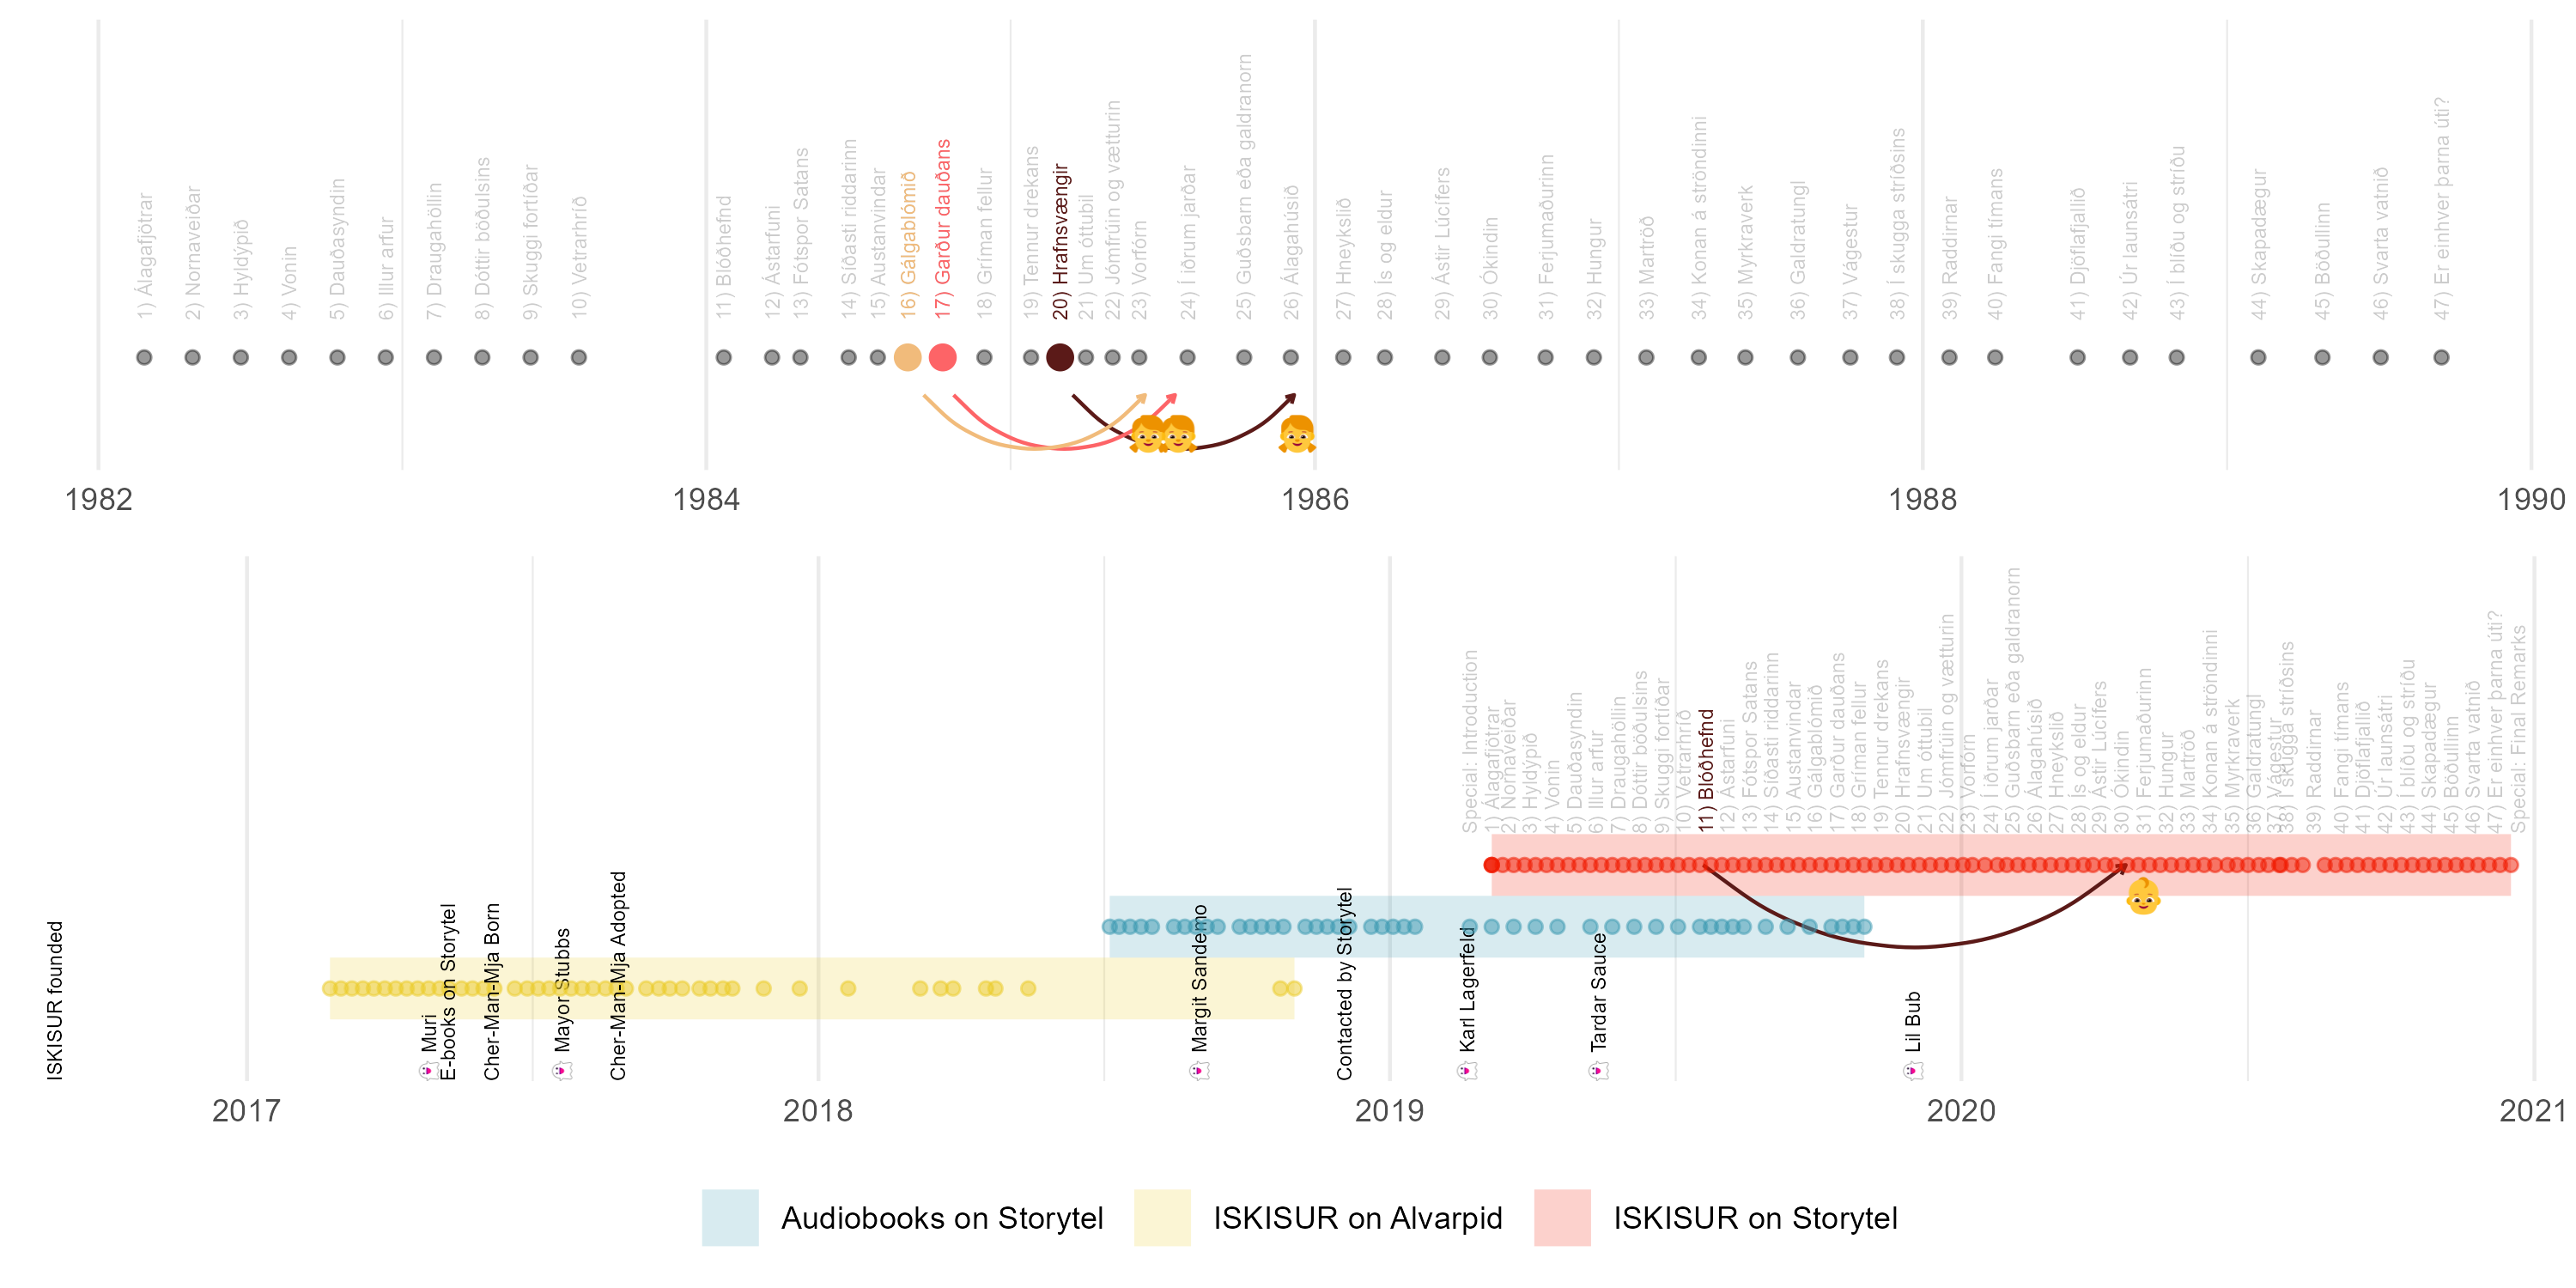
\includegraphics[width=\textwidth]{../rek-data-beers/R/figures/timeline}
\end{frame}
